% sections/results_b.tex
% Results R4-R6. Continues \section{Results} opened in sections/results_a.tex;
% do not re-issue \section{Results} here. results/ is empty and the campaign
% is re-running -- every quantity below is \nm{...}; every speculative
% sentence is wrapped in \spec{...}. See NARRATIVE.md \S12 for the Table 1
% restructuring this file implements (deployed end-to-end headline column,
% best-cell oracle as a labelled upper bound, gap = regret).

\subsection*{The winning representation pairing migrates across real corpora}
\label{sec:r4}

The sweeps in the preceding subsections vary density and working-set size by
construction, and a generator can always be suspected of encoding exactly the
structure its own kernels are built to exploit. We therefore repeated the
central comparison on corpora with independent provenance: the twelve corpora
CRoaring's own benchmark harness runs by default \cite{chambi2016roaring,lemire2018roaring},
together with \prov{five} larger modern graphs, for \prov{17} corpora spanning
\prov{$7.89\times10^{-7}$ to $1.73\times10^{-1}$} in density and
\prov{$1.995\times10^{5}$ to $3.697\times10^{7}$} bits in universe size
(Supplementary Table~\ref{tab:corpus-inventory} lists the provenance of every
corpus, including the further corpora scored only against an all-bitmap
baseline, never against CRoaring). Every corpus in this seventeen-corpus set
is scored against the same \texttt{run\_optimize()}-tuned CRoaring baseline
used throughout Results, so this comparison is continuous with, not separate
from, the synthetic sweeps above.

Table~\ref{tab:corpora} reports, for every corpus, its universe size and
density, the pairing cell that won on it, and two ratios against a baseline.
\textbf{Both ratios are best-cell, oracle selection} -- hindsight choice of
representation pairing, no selection cost charged -- \textbf{not the deployed
selector run end to end.} That end-to-end number does not exist yet:
\texttt{results/} has been cleared and the campaign that will produce it is in
flight (Methods). Presenting an oracle ratio without labelling it as such would
violate this paper's own standard (Limitations, L7), so every ratio column in
Table~\ref{tab:corpora} is headed \emph{oracle}, and closing the gap to a
deployed, charged selector -- the same regret quantity reported in aggregate
above (Fig.~\ref{fig:selection-cost}) -- is stated as the immediate next step
in Discussion rather than shown as a second column here. Storm's best cell
beat tuned CRoaring on \prov{17 of 17} corpora tested, ratio range
\prov{$1.12\times$ to $16.06\times$}, median \prov{$\approx 6.1\times$} --
excluding \texttt{uscensus2000} and \texttt{dimension\_033}, which the
measurement-drift caveat below flags as unquotable at this precision (their
density and winning cell are still shown; only their ratio cells are
suppressed). Per-corpus ratios are reported to two decimal places because
that is the precision the retired campaign's source table carries, \textbf{not
because they are trustworthy to that precision}: the campaign ran as a single
back-to-back batch rather than round-robin-interleaved repeats, so every ratio
here should be read as a point estimate with an unquantified spread of at
least $\pm 1$ significant figure (Methods; repeated in the caption).

More informative than either ratio is which cell wins where. Across the
seventeen-corpus set, \prov{$\cell{\rB}{\rB}$ wins 10, $\cell{\rB}{\rS}$ wins
3, $\cell{\rB}{\rR}$ wins 2, $\cell{\rS}{\rS}$ wins 1, and $\cell{\rR}{\rR}$
wins 1} -- no single cell accounts for a plurality of the corpora, let alone
all of them. Had one cell dominated that count, the pairing matrix would have
had nothing left to select among, and this result would have refuted the
paper's own thesis; it does not, and the winner instead tracks each corpus's
density, exactly as the density sweep above predicts (Table~\ref{tab:corpora}).

The migration is expected to follow the same axis established synthetically
above. \spec{If the real corpora behave like the density sweep, corpora at
the sparse end should be won by array- and rank-based cells such as
$\cell{\rB}{\rS}$ and $\cell{\rB}{\rR}$, dense corpora by $\cell{\rB}{\rB}$,
and clustered or highly skewed corpora by run-based cells such as
$\cell{\rR}{\rR}$ -- the same three regimes the U-shaped curve predicts, now
read off independently sourced data rather than a generator.} \spec{The
fill-compressed cell, $\cell{\rW}{\rW}$, is likewise expected to remain the
consistent loser here, as it was in the synthetic sweeps above:} it
underperforms the tuned baseline on \prov{16 of 17} corpora,
\spec{which if it reproduces would be the clearest
real-data instance of the cost of choosing wrong that this paper argues
throughout}. Taken together, the migration and the histogram are the result
reported here -- not a ratio, but a map of which representation is correct
for which corpus, read directly off data whose structure this project did not
generate.

\begin{table}[!t]
\scriptsize
\setlength{\tabcolsep}{2.2pt}
\renewcommand\arraystretch{1.05}
\centering
\caption{\textbf{The winning representation pairing migrates with corpus
density.} \textbf{\textcolor{red}{Superseded: the CRoaring column is measured against an
under-tuned baseline.}} A twenty-line change to CRoaring --- promoting array containers above
cardinality~64 to bitsets after \texttt{run\_optimize()} --- removes most of the dense-corpus
advantage shown here (\texttt{census1881} $13.4\times \to 0.59\times$; \texttt{census-income}
$10.7\times \to 1.88\times$), while sparse-corpus results are untouched or improve. What is withdrawn is a
\emph{kernel-level} advantage, which was never the contribution: with the meta-filter layer applied
on top, the result stands against the repaired baseline. Every CRoaring value below must be
re-derived against \emph{both} baselines before this table is quoted. \prov{14 of 23} real corpora (Methods, ``Corpora, provenance and
loaders''; full inventory in Supplementary Table~\ref{tab:corpus-inventory}),
grouped by density band, chosen to span every domain in the set and both
speedup extremes; the remaining \prov{9} corpora are summarized in the final
row. A further, non-benchmark-set corpus (\texttt{1KGP3 chr20},
haplotype-major) is shown in the Mixed band because it is this paper's own
stated counterexample (Limitation L2) and must not be omitted for being
unflattering. \textbf{Both ratio columns are oracle}: best-cell selection with
hindsight, no selection cost charged --- not the deployed, end-to-end
selector, which does not yet exist (\texttt{results/} was cleared for the
current campaign; Discussion). ``vs.\ CRoaring'' is against a
\texttt{run\_optimize()}-tuned baseline \cite{chambi2016roaring,lemire2018roaring};
``vs.\ all-bitmap'' is context only and is \emph{not} always from the same
measurement campaign as the CRoaring column (marked \dag/\ddag/\S below), so
the two ratio columns in a single row should not be assumed comparable to each
other. \textbf{All values are provisional, from a retired measurement
campaign} (orange) and are not trustworthy to the two- or three-significant-
figure precision shown --- report medians and ranges, not individual cells, in
prose. $^\dagger$ \texttt{uscensus2000} and \texttt{dimension\_033}: ratio cells
suppressed and excluded from every headline range above; unlike the other
excluded corpora discussed in Methods, the \emph{winning cell itself} moved
between repeats for these two (not only the magnitude), so the cell shown is
the retired campaign's single run, not a stable result, and is not to be read
as settled. Density is a corpus property, not a per-run measurement, and is
unaffected. $^\ddagger$ vs.\
all-bitmap only, from the default-selection benchmark (main README ``Results''
table), not the CRoaring head-to-head campaign; no oracle-vs-CRoaring value
exists for this row. $^\S$ scoping corpus, not part of the 23-corpus set;
ratio below $1.0\times$ means all-bitmap beats selection outright at this
density and (haplotype-major) layout --- the honest reading is a loss, not a
rounding artefact. ---, not applicable. Winning cell in bold.}
\label{tab:corpora}
\begin{tabular}{@{}c | l l S[table-format=1.2e1] S[table-format=1.2e-1] l S[table-format=2.2] S[table-format=5.2]@{}}
\toprule
& Corpus & Domain & {Universe $m$ (bits)} & {Density} & Winning cell & {vs.\ CRoaring (oracle, $\times$)} & {vs.\ all-bitmap ($\times$)} \\
\midrule
\multirow{7}{*}{Sparse}
& \texttt{enwiki-categorylinks} & IR      & {1.30e8} & {7.89e-7} & {\nm{cell}} & {\nm{n/a}} & {\prov{1083}$^\ddagger$} \\
& \texttt{uscensus2000}$^\dagger$ & census & {3.70e7} & {8.09e-7} & {\prov{B$\times$S}$^\dagger$} & {$^\dagger$} & {$^\dagger$} \\
& \texttt{dbpedia-link}         & graph   & {1.83e7} & {1.63e-6} & {\nm{cell}} & {\nm{n/a}} & {\prov{311}$^\ddagger$} \\
& \texttt{as-skitter}           & graph   & {1.70e6} & {9.08e-6} & \textbf{\prov{B$\times$S}} & {\textbf{\prov{4.02}}} & {\prov{756}} \\
& \texttt{wiki-Talk}            & graph   & {2.39e6} & {2.17e-5} & \textbf{\prov{B$\times$S}} & {\textbf{\prov{8.80}}} & {\prov{910}} \\
& \texttt{gnomad\_chr21\_exomes\_af1e-3} & genomics & {1.46e6} & {1.93e-5} & {\nm{cell}} & {\nm{n/a}} & {\prov{222}$^\ddagger$} \\
& \texttt{dimension\_008}       & druid   & {3.87e6} & {8.98e-5} & \textbf{\prov{R$\times$R}} & {\textbf{\prov{1.73}}} & {\prov{2846}} \\
\cmidrule(lr){2-8}
\multirow{5}{*}{Mixed}
& \texttt{usher\_sarscov2}      & genomics & {8.45e6} & {1.87e-3} & {\nm{cell}} & {\nm{n/a}} & {\prov{121}$^\ddagger$} \\
& \texttt{wikileaks-noquotes}   & text    & {1.35e6} & {1.02e-3} & \textbf{\prov{B$\times$B}} & {\textbf{\prov{6.79}}} & {\prov{67}} \\
& \texttt{census1881}           & census  & {4.28e6} & {1.17e-3} & \textbf{\prov{B$\times$B}} & {\textbf{\prov{16.06}}} & {\prov{151}} \\
& \texttt{dimension\_033}$^\dagger$ & druid & {3.87e6} & {5.78e-3} & {\prov{B$\times$R}$^\dagger$} & {$^\dagger$} & {$^\dagger$} \\
& \texttt{1KGP3 chr20} (hap.-major)$^\S$ & genomics & {1.05e6} & {3.1e-2} & \textbf{\prov{B$\times$B}} & {\nm{n/a}} & {\prov{0.93}$^\S$} \\
\cmidrule(lr){2-8}
\multirow{3}{*}{Dense}
& \texttt{weather\_sept\_85}    & sensor  & {1.02e6} & {6.34e-2} & \textbf{\prov{B$\times$B}} & {\textbf{\prov{15.02}}} & {\prov{2}} \\
& \texttt{msprime\_10k}         & genomics-sim & {2.00e4} & {9.4e-2} & {\nm{cell}} & {\nm{n/a}} & {\prov{2}$^\ddagger$} \\
& \texttt{census-income}        & census  & {2.00e5} & {1.73e-1} & \textbf{\prov{B$\times$B}} & {\textbf{\prov{13.11}}} & {\prov{1}} \\
\addlinespace
& \multicolumn{2}{l}{remaining \prov{9} corpora (Supp.\ Table~\ref{tab:corpus-inventory})} & {---} & {\prov{4.15e-6--7.9e-2}} & varies & {\prov{1.12--6.07}} & {\prov{3--523}} \\
\bottomrule
\end{tabular}
\end{table}

\subsection*{Fixed chunk granularity misprices dense corpora}
\label{sec:r5}

Although representation selection beats tuned CRoaring on nearly every corpus
tested above, several corpora at moderate-to-high global density --
\prov{$1.2\times10^{-3}$ to $1.7\times10^{-1}$} -- show CRoaring
losing by more than an identically dense popcount workload should explain. We
diagnosed the gap using CRoaring's own instrumentation rather than ours:
Table~\ref{tab:census} gives, per corpus, the array, bitset and run containers
a \texttt{run\_optimize()}-tuned CRoaring bitmap settles on, taken after tuning
so that the census reflects how the library is actually deployed (Methods,
``Container census'').

CRoaring's container choice is a per-chunk, fixed-threshold rule, read from the
vendored library rather than measured by us: each $2^{16}$-bit chunk is stored
as an array container unless that chunk's own cardinality exceeds a
compile-time constant (Methods, ``Container census''). On
\texttt{census1881} at \prov{$1.2\times10^{-3}$} global density, the tuned
bitmap contains \prov{1{,}332} array containers against \prov{\textbf{0}}
bitset containers and \prov{132} run containers, out of \prov{1{,}464} chunks
(Table~\ref{tab:census}) -- essentially no chunk ever crosses the threshold,
despite the corpus being dense by any global measure. \spec{Because the
threshold test is corpus-independent -- it only ever inspects one chunk's own
cardinality -- the same mispricing should reproduce on any corpus whose mass
is large enough, and spread thinly enough, to keep every individual chunk
under the threshold while the corpus as a whole is unambiguously dense; the
other rows of Table~\ref{tab:census} are included to check whether that
prediction holds beyond the single sharpest case.}

The mechanism is that a fixed per-chunk threshold is tested against the wrong
statistic. With a large universe, a corpus's mass can spread across enough
chunks that every individual chunk stays under the threshold even while global
density reaches \prov{6.3\% (\texttt{weather\_sept\_85}) or 17.3\%
(\texttt{census-income})}, so CRoaring runs array merges where a bitmap popcount would be
strictly cheaper. This is not evidence that CRoaring is poorly engineered: it
is evidence that a threshold chosen once, at ingest, for a workload built
around a single pairwise operation cannot be correct for every global density
a corpus might later be evaluated at -- precisely the fixed-granularity
limitation this paper's opening names and the results above are built to work
around.

\begin{table}[!t]
\footnotesize
\setlength{\tabcolsep}{6pt}
\renewcommand\arraystretch{1.05}
\centering
\caption{\textbf{Roaring's fixed per-chunk threshold is tested against the
wrong statistic.} Container composition of a \texttt{run\_optimize()}-tuned
CRoaring bitmap \cite{chambi2016roaring,lemire2018roaring}, counted after
tuning (Methods, ``Container census''), for the \prov{four} corpora of
Table~\ref{tab:corpora} the retired campaign ran a container census on --
\prov{three} from the Mixed/Dense bands plus \texttt{uscensus2000} from the
Sparse band, kept in \emph{despite} its extreme sparsity because it shows the
same array-container plurality persists even there. Roaring assigns a bitset
container to a $2^{16}$-bit chunk only when that chunk's own cardinality
exceeds a fixed compile-time constant \prov{(4096, per vendored source; tier 2,
a vendor fact, not a measurement of ours)} --- a per-chunk statistic, not the
corpus's global density --- so a corpus that is dense in aggregate can receive
almost no bitset containers. Global density is the fraction of the shared
universe set across the whole corpus. \textbf{Total chunks} is the sum of the
three container counts (every non-empty $2^{16}$-bit chunk across the
corpus's bitmaps), not an independently measured quantity. Bold marks the
plurality container type per row; all four rows are plurality-array, which is
the finding. All values \prov{provisional, retired campaign}. ---, not
applicable.}
\label{tab:census}
\begin{tabular}{@{}l S[table-format=1.2e-1] S[table-format=5.0] S[table-format=5.0] S[table-format=5.0] S[table-format=5.0]@{}}
\toprule
Corpus & {Global density} & {Array containers} & {Bitset containers} & {Run containers} & {Total chunks} \\
\midrule
\texttt{uscensus2000}   & {\prov{8.1e-7}} & {\textbf{\prov{2219}}} & {\prov{0}} & {\prov{2}} & {\prov{2221}} \\
\texttt{census1881}     & {\prov{1.2e-3}} & {\textbf{\prov{1332}}} & {\prov{0}} & {\prov{132}} & {\prov{1464}} \\
\texttt{weather\_sept\_85} & {\prov{6.3e-2}} & {\textbf{\prov{2274}}} & {\prov{561}} & {\prov{21}} & {\prov{2856}} \\
\texttt{census-income}  & {\prov{1.7e-1}} & {\textbf{\prov{553}}} & {\prov{180}} & {\prov{35}} & {\prov{768}} \\
\bottomrule
\end{tabular}
\end{table}


Two mechanisms serve the thresholded mode, and the cheaper of them touches no data whatsoever.
Because $|A \cap B| \le \min(a,b)$ while $|A \cup B| \ge \max(a,b)$, a pair's similarity is capped by
the ratio of its two sizes, $J(A,B) \le \min(a,b)/\max(a,b)$, so a pair whose sizes differ by more
than a factor $1/t$ cannot reach the threshold and is discarded from two integers, before either
operand is read. An absolute threshold behaves the same way: $|A \cap B| \ge \tau$ requires only
$\min(a,b) \ge \tau$. Restricting the \emph{inputs} to a band of sizes --- ignoring the extremely
rare, or keeping only those --- is that same comparison applied before a pair is formed rather than
after. The bound is the Swamidass--Baldi pruning result \cite{swamidass2007bounds} together with the
size filter of the similarity-join literature \cite{bayardo2007allpairs,xiao2008ppjoin}; what is
reported here is not the bound but where it sits relative to the rest and how it composes with them.

How much it removes is fixed by one property of the corpus, and that property is what makes it worth
separating from the mechanisms above. Under the $1/i$ cardinality spectrum this paper benchmarks ---
cardinalities log-uniform on $[1,K]$, which is the density $\Pr(a) \propto 1/a$ exactly, so this is
the mandated spectrum and not a stand-in for it --- the fraction of pairs that can possibly qualify
is $1 - (1 - \ln(1/t)/\ln K)^{2}$ (Methods, Eq.~\eqref{eq:survive}), which agrees with a $10^{5}$-sample
simulation to three decimals. At $K = 10^{4}$ that leaves $14.5\%$ of pairs at $t = \tfrac12$,
$4.8\%$ at $t = 0.8$, $2.3\%$ at $t = 0.9$ and $1.1\%$ at $t = 0.95$, so examining every pair does
$6.9\times$ to $90.0\times$ the work of examining only the survivors. \textbf{The expression falls
as $K$ rises: the wider the spread of set sizes, the more pairs are ruled out by the ratio alone.}
That is the reverse of the dependence every other mechanism here has. The null models of
Fig.~\ref{fig:density-sweep} are all stated at a \emph{fixed} density and bound what a mechanism is
worth against within-row arrangement; the size bound is the only one whose value is a function of
the \emph{dispersion of cardinalities across the corpus}, and it strengthens monotonically as that
dispersion widens --- $2.3\%$ surviving at $K = 10^{4}$ against $1.1\%$ at $K = 10^{8}$, both at
$t = 0.9$. The two axes are different and not in competition. One limit is worth stating with it:
the favourable scaling belongs to this spectrum rather than to skew in general, and under a heavier
tail in which \emph{ranked} sizes scale as $1/i$ the surviving fraction is exactly $1 - t$ whatever
$K$ is (Methods).

It does not, however, multiply with the mechanisms below it, and the reason refines the composition
rule this section has otherwise used. Deciding whether a pair exists at all is the coarsest
granularity in the paper, so the rule as stated predicts a clean product with anything acting inside
a pair. The product is not achieved. The survivors of the size test are the pairs with $a \approx b$,
and representation choice, a zone map and the prefix filter are each cheapest precisely when the two
sizes are \emph{dissimilar} --- so the test passes on the pairs the rest serve worst, and the
composed cost exceeds the product of the two savings by the factor that conditioning raises a
survivor's mean cost, $\ln K / 2$ in the limit of a high threshold (Methods,
Eq.~\eqref{eq:shortfall}). At $K = 10^{4}$, $t = 0.9$ and $m = 10^{6}$ the size bound leaves
$2.76\%$ of pairs and representation choice costs $1.51\%$ of a bitmap, so a product would predict
$0.042\%$ where the composition costs $0.151\%$. Replaying the same composition with the size test
decorrelated from cardinality, at an identical survival rate, restores the product to within
$0.6\%$, which identifies the shared statistic rather than the shared granularity as the cause. The
composition remains firmly worth taking --- it costs $10.0\%$ of the better of the two mechanisms
alone, and a bitmap pass over every pair does $660\times$ its work --- so what this refutes is the
product, not the composition. \textbf{Mechanisms compose multiplicatively when they act on different
waste \emph{and} read different operand statistics; acting at different granularities is necessary
and not sufficient.} These are analytic values over the model above, and like the rest of this
section they count work rather than time.

The thresholded mode changes the contract rather than the kernel: only pairs above a similarity
threshold are reported, and the second mechanism that exploits that is prefix filtering rather than
any representation choice. It admits the same analysis, and it reduces further than the others do.
Because a qualifying pair must share an element between its prefixes, the entire behaviour of the
filter is governed by one dimensionless quantity --- the expected number of shared prefix elements
per pair, $y = p^{2}/m$ --- and the fraction of pairs surviving is $1 - e^{-y}$ regardless of
density, threshold or universe size separately (Fig.~\ref{fig:prefix}). Below $y = 1$ pruning
improves quadratically as prefixes shorten; above it prefixes collide by default and the index earns
nothing. \spec{That single variable is what a gate for this mode should test, and it is cheap to
compute from the metadata already held.}


\begin{figure}[!t]
\centering
\textbf{a}\par\vspace{0.6mm}
% Prefix-filtering schematic (was Fig. 1e)
% Extracted from the former Fig. 1; rendered as a panel of its own figure.
\centering
% ===========================================================================
% Figure 1 — overview. Body only; \input inside a figure environment.
% House idiom follows the scaffold paper's fig:planes: minipage panels with
% bold letter labels, \resizebox per panel, and the two-saturation convention
% (strong fill = the lanes the panel is about, faint same-hue fill = context).
%
% Requires simdgrid.sty and the repr* colours from storm.tex.
% ===========================================================================

% Focus / context saturations, one pair per representation.
\colorlet{focB}{reprB!45}\colorlet{ctxB}{reprB!12}
\colorlet{focS}{reprS!55}\colorlet{ctxS}{reprS!14}
\colorlet{focR}{reprR!55}\colorlet{ctxR}{reprR!14}
\colorlet{focW}{reprW!55}\colorlet{ctxW}{reprW!14}
\colorlet{focC}{reprC!65}\colorlet{ctxC}{reprC!18}
\colorlet{zone}{black!18}

\tikzset{
  gridcell/.style={draw=black!55, line width=0.4pt, minimum width=16.5mm,
                   minimum height=6.6mm, inner sep=1pt, font=\scriptsize,
                   anchor=center},
  hdr/.style={font=\scriptsize\bfseries},
  flowbox/.style={draw=black!60, rounded corners=1.2pt, align=left,
                  font=\scriptsize, inner sep=3.2pt},
  flowarrow/.style={-{Latex[length=1.8mm]}, draw=black!65, line width=0.5pt},
}

% ------------------------------------------------------------------ panel e
% Prefix filtering: a candidate-pruning rule from the similarity-join
% literature, used only in the opt-in thresholded mode.
\centering
\resizebox{.23\linewidth}{!}{%
\begin{tikzpicture}[x=1mm,y=1mm]
  \tikzset{sm/.style={draw=black!55, line width=0.35pt},
           tiny lbl/.style={font=\scriptsize, text=black!70}}
  % Type size: cell values were \tiny against \scriptsize row labels, and the
  % whole picture was then scaled up ~1.9x, so the labels rendered about 15 pt
  % -- larger than the body text and roughly four times the neighbouring
  % matplotlib panels. Every glyph is \scriptsize now and the picture is set
  % near its natural size, so it renders at ~8 pt like everything around it.
  % Encoding, not prose: prefix = saturated, tail = near-white, the shared
  % element = accent. The verdict is a glyph. The caption narrates.
  %
  % Prefix-versus-tail is a pure LUMINANCE axis (mid ink against near-white),
  % so it survives greyscale on its own and costs no hue. It used to be drawn
  % in S's blue and the shared element in R's green, which spent two
  % representation hues on things that are not representations. The shared
  % element is what makes the pair survive to exact verification, so it now
  % takes the same reserved "work" accent used everywhere else in the paper,
  % and the discarded pair takes the "work avoided" accent.
  \definecolor{workc}{HTML}{EE6677}
  \definecolor{avoidc}{HTML}{66CCEE}
  \colorlet{pfx}{black!26}\colorlet{tail}{black!5}\colorlet{hit}{workc}
  \newcommand{\prefrow}[5]{% #1 y  #2 label  #3 prefix  #4 tail  #5 hit index (-1 none)
    \node[font=\scriptsize\bfseries, anchor=east] at (-1.4,#1+2.1) {#2};
    \foreach \v [count=\k from 0] in {#3}{
      \ifnum\k=#5 \def\f{hit}\else\def\f{pfx}\fi
      \draw[sm, fill=\f] (\k*5,#1) rectangle ++(5,4.2);
      \node[font=\scriptsize\bfseries] at (\k*5+2.5,#1+2.1) {\v};}
    \foreach \v [count=\k from 0] in {#4}{
      \draw[sm, draw=black!35, fill=tail] (\k*5+10,#1) rectangle ++(5,4.2);
      \node[font=\scriptsize, text=black!45] at (\k*5+12.5,#1+2.1) {\v};}}
  % verdict glyphs, drawn rather than set as text
  \newcommand{\vdiscard}[2]{\draw[line width=1.1pt, draw=avoidc!55!black]
      (#1-1.7,#2-1.7) -- (#1+1.7,#2+1.7) (#1-1.7,#2+1.7) -- (#1+1.7,#2-1.7);}
  \newcommand{\vkeep}[2]{\draw[line width=1.2pt, draw=workc!65!black,
      line cap=round,
      line join=round] (#1-1.9,#2+0.1) -- (#1-0.5,#2-1.5) -- (#1+2.0,#2+1.9);}

  \draw[-{Latex[length=1.3mm]}, draw=black!45, line width=0.4pt] (0,10.4) -- (10,10.4);
  \node[font=\scriptsize, text=black!55, anchor=west] at (10.8,10.4) {rarest first};
  \prefrow{0}{$A$}{17,4}{23,8,31}{-1}
  \prefrow{-6}{$B$}{12,23}{8,31,5}{-1}
  \draw[decorate, decoration={brace, amplitude=2.2pt}, draw=black!55]
    (0,4.7) -- (10,4.7) node[midway, above=1.8pt, font=\scriptsize, text=black!65] {prefix};
  \vdiscard{31}{-3}

  \begin{scope}[shift={(0,-11.5)}]
    \prefrow{0}{$A$}{17,4}{23,8,31}{1}
    \prefrow{-6}{$C$}{4,12}{8,31,5}{0}
    \vkeep{31}{-3}
  \end{scope}
\end{tikzpicture}}


\vspace{2mm}
\par\vspace{1.5mm}
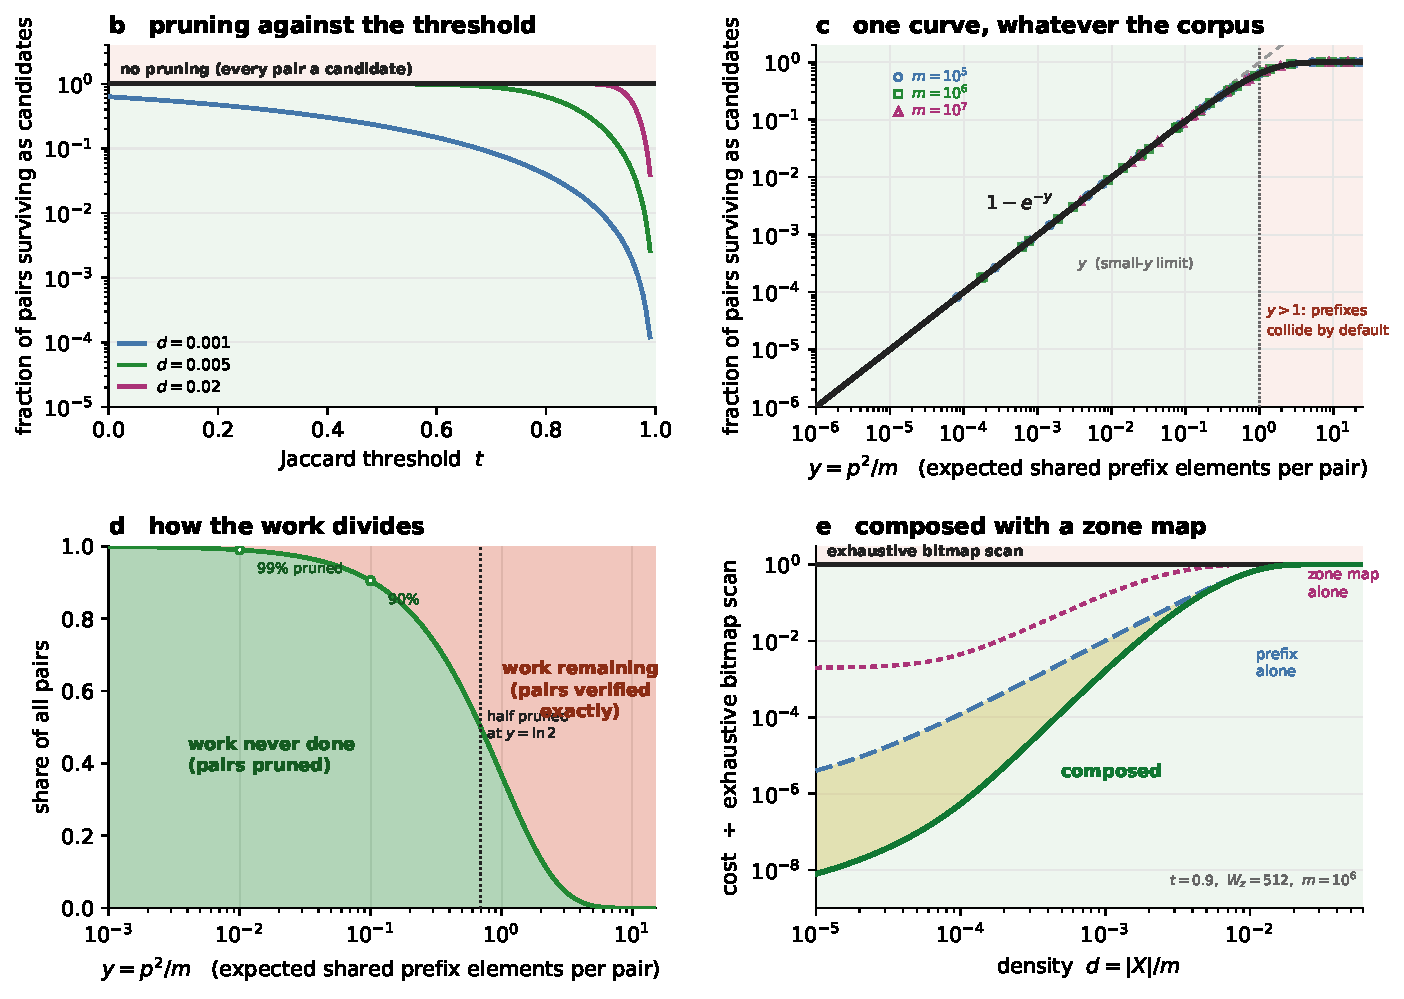
\includegraphics[width=.94\linewidth]{figures/fig3_prefix}
\caption{\textbf{Prefix filtering, analysed on the same terms --- and reducible to a single
variable.} Prefix filtering serves the opt-in thresholded mode, in which only pairs of Jaccard
similarity at least $t$ are reported. With elements in a global order and prefix length
$p(X) = |X| - \lceil t|X| \rceil + 1$, any qualifying pair must share an element between its
prefixes, so indexing prefixes alone answers the thresholded question exactly. Unlike the mechanisms
of Fig.~\ref{fig:pairing-matrix}c--d it is candidate \emph{generation}: the quadratic pair set is
never enumerated.
\textbf{a}, How the rule works. Elements are laid out in a global order --- by document frequency,
rarest first, hence the non-monotonic labels --- and each set's prefix (saturated, bold) is its
rarest $p(X)$ elements, a length that depends on $t$; the remainder is greyed. Any pair with
$J(A,B)\ge t$ must share at least one element between its prefixes. Top: the prefixes have no
element in common, so the pair is discarded without computing any intersection. Bottom: one element
(green) appears in both, so the pair becomes a candidate and is verified exactly.
\textbf{b}, Fraction of pairs surviving as candidates against the threshold, at universe $10^{6}$.
Pruning is governed by how long the prefixes are, and prefix length falls as $t$ rises, so the same
filter that removes almost everything at a high threshold removes almost nothing at a low one --- and
denser operands need a higher threshold to reach the same pruning.
\textbf{c}, All of that collapses onto one curve. For prefixes of length $p$ over a universe of $m$
the expected number of shared prefix elements per pair is $y = p^{2}/m$, and the surviving fraction
is exactly $1 - e^{-y}$ for scattered operands; markers are $(d,t,m)$ combinations drawn at random
across three universe sizes, and they lie on the curve by construction rather than by fit. Two
regimes follow. For $y \ll 1$ the surviving fraction is $y$ itself, so pruning improves
\emph{quadratically} as prefixes shorten. For $y > 1$ prefixes collide by default, essentially every
pair is a candidate, and the index is pure overhead --- the same shape of liability as a summary too
sparse to pay for itself (Fig.~\ref{fig:density-sweep}). The useful operating region is therefore
$y \ll 1$, and $y$ --- not $t$, and not density --- is the quantity a selector should test.
\textbf{d}, The same information as a division of labour: on a linear axis, the share of all pairs
never examined against the share surviving to exact verification. The two are equal at $y = \ln 2$.
\textbf{e}, Prefix filtering composed with a zone map. Unlike the two mechanisms of
Fig.~\ref{fig:density-sweep}c, these \emph{do} compose --- their savings multiply, and the composed
curve tracks the product of the two to within \nm{a factor of 1.25 at the sparsest end, exactly
elsewhere; analytic}. The reason is that they act on different waste \emph{and} read different
statistics of the operands: prefix filtering decides \emph{which} pairs are examined at all, from
element identity, while a zone map reduces the work \emph{within} a pair, from bin occupancy. Both
conditions are needed. Where two mechanisms attack the same waste --- as a zone map and a
representation both do inside one pair --- filtering concentrates what it passes on and the
composition is worth far less than the product; and where two mechanisms read the same statistic,
the second inherits a biased sample from the first even when their granularities differ. At $d = 10^{-3}$, $t = 0.9$ and $W_z = 512$ the composition costs
\nm{$\approx 0.17\%$, analytic} of an exhaustive bitmap scan, against $1.0\%$ for prefix filtering
alone and $16\%$ for a zone map alone.
Analytic throughout; this figure contains no measured data, and like Fig.~\ref{fig:density-sweep} it
models work rather than time. \spec{Real corpora deviate from it in the same direction as elsewhere:
frequency-ordered prefixes concentrate rare elements, so real prefixes collide less than scattered
ones of the same length and the true curve lies below this one.}}
\label{fig:prefix}
\end{figure}

\subsection*{Where the method does not pay}
\label{sec:r6}

Although the best cell beat tuned CRoaring on \prov{17 of 17} corpora tested
above (oracle selection; Table~\ref{tab:corpora}), it does not win
everywhere, and the domain it wins on is worth stating precisely rather than
implying it is universal. The first boundary is the one already drawn by the
density sweep earlier in Results: between the two crossovers sits a band
where nothing beats $\cell{\rB}{\rB}$, and the corpus set above confirms real
data lands there too -- \prov{10 of 17} real corpora are won by
$\cell{\rB}{\rB}$ itself. Reporting that band as a shortfall would misstate the
finding: inside it, the method's job is to recognize the band cheaply and
step aside, not to outperform a kernel that is already optimal there. The
second boundary is that layout, not only content, determines which regime a
dataset falls into. The same genomic cohort sits deep in the sparse regime in
variant-major orientation -- \prov{121--222$\times$} against an all-bitmap
baseline (\texttt{usher\_sarscov2}, \texttt{gnomad\_chr21\_exomes\_af1e-3};
no CRoaring comparison exists for these two) -- but in
haplotype-major orientation lands inside the mid-band, where all-bitmap wins
outright, \prov{0.93$\times$} (\texttt{1KGP3 chr20}, hap.-major; Limitation
L2). This paper does not choose
the orientation a downstream dataset arrives in, and real data gives a large
universe or sparsity far more often than both together.

The third boundary is the selector's own maturity: as established above,
nothing measured in this campaign closes the residual gap to the bucket
oracle. Selection here is cheap, not optimal. None of these three
boundaries undermines the result reported above; together they define its
domain -- representation selection wins broadly, on a stated and bounded
range of corpus shapes, with a known and disclosed edge.

\subsection*{Supplementary tables}
\label{sec:supp-tables}

Storage is a reported trade-off, not an objective this paper optimizes for
(Discussion), so the following three tables are supplementary rather than
main-text, per the display-item allocation (\texttt{NARRATIVE.md} \S7). No
dedicated supplementary file exists yet in this draft; they are placed here,
clearly labelled, until one is built.

% longtable is NOT a float and creates no group, so a bare \scriptsize here
% leaks into every following section. Keep it inside an explicit group.
\begingroup
\scriptsize
\setlength{\tabcolsep}{2.2pt}
\begin{longtable}{@{}p{2.9cm} l r r r r p{4.3cm}@{}}
\caption{\textbf{Supplementary Table S1 | Corpora, provenance and statistics.}
Every corpus referenced anywhere in this paper, in the four provenance groups
used to assemble the benchmark set: \textbf{G1}, the twelve
\texttt{real-roaring-datasets} files CRoaring's own harness runs by default
\cite{chambi2016roaring,lemire2018roaring}; \textbf{G2}, five SNAP social/web
graphs (Stanford Large Network Dataset Collection) scored by
neighbourhood-intersection density; \textbf{G3}, two genomic corpora \emph{present for
scoping, not for the headline} -- included specifically so a reader can judge
whether the benchmark set was chosen favourably, per the standing reviewer
question this table exists to pre-empt; \textbf{G4}, KONECT graphs, UShER
SARS-CoV-2, gnomAD and the \texttt{msprime} coalescent-simulation series,
added after the original survey. Density and mean $|X_i|$ are corpus
properties from the data loaders, not timing results, and are consequently
far more stable than any ratio in Tables~\ref{tab:corpora}--\ref{tab:census}
-- but they still originate in the retired campaign and are marked
provisional like every other number in this draft. For the two G3 corpora,
\emph{universe} and \emph{rows} swap roles between layouts: \texttt{chr20.bin}
is variant-major (universe = 5{,}008 haplotypes, one row per variant site);
\texttt{chr20\_hap.bin} is haplotype-major (universe $\approx$ 1{,}048{,}576
sites, one row per haplotype) -- the layout dependence that Limitation L2 is
about. ---, not reported by the source.}
\label{tab:corpus-inventory}\\
\toprule
Corpus & Group & Rows/sets & Universe $m$ & Mean $|X_i|$ & Density & Origin / notes \\
\midrule
\endfirsthead
\multicolumn{7}{l}{\textit{Supplementary Table S1 (continued)}} \\
\toprule
Corpus & Group & Rows/sets & Universe $m$ & Mean $|X_i|$ & Density & Origin / notes \\
\midrule
\endhead
\midrule \multicolumn{7}{r}{\textit{continued on next page}} \\
\endfoot
\bottomrule
\endlastfoot
\texttt{\seqsplit{census1881}} & G1 & \prov{200} & \prov{4{,}277{,}806} & \prov{5{,}019} & \prov{1.2e-3} & 1881 Canadian census, categorical attributes \\
\texttt{\seqsplit{census1881\_srt}} & G1 & \prov{200} & \prov{4{,}277{,}735} & \prov{3{,}404} & \prov{8.0e-4} & as above, rows sorted \\
\texttt{\seqsplit{census-income}} & G1 & \prov{200} & \prov{199{,}523} & \prov{34{,}610} & \prov{1.7e-1} & US census income (UCI ``Adult''-family), attributes \\
\texttt{\seqsplit{census-income\_srt}} & G1 & \prov{200} & \prov{199{,}523} & \prov{30{,}464} & \prov{1.5e-1} & as above, rows sorted \\
\texttt{\seqsplit{weather\_sept\_85}} & G1 & \prov{200} & \prov{1{,}015{,}367} & \prov{64{,}353} & \prov{6.3e-2} & September 1985 weather observations, binned attributes \\
\texttt{\seqsplit{weather\_sept\_85\_srt}} & G1 & \prov{200} & \prov{1{,}015{,}367} & \prov{80{,}540} & \prov{7.9e-2} & as above, rows sorted \\
\texttt{\seqsplit{wikileaks-noquotes}} & G1 & \prov{200} & \prov{1{,}353{,}179} & \prov{1{,}377} & \prov{1.0e-3} & WikiLeaks cable corpus, term/attribute postings \\
\texttt{\seqsplit{wikileaks-noquotes\_srt}} & G1 & \prov{200} & \prov{1{,}353{,}133} & \prov{1{,}440} & \prov{1.1e-3} & as above, rows sorted \\
\texttt{\seqsplit{uscensus2000}} & G1 & \prov{200} & \prov{36{,}974{,}578} & \prov{30} & \prov{8.1e-7} & US Census 2000; \textbf{sparsest and largest-universe G1 corpus} \\
\texttt{\seqsplit{dimension\_003}} & G1 & \prov{15{,}482} & \prov{3{,}866{,}847} & \prov{91} & \prov{2.4e-5} & Druid-derived dimension column \\
\texttt{\seqsplit{dimension\_008}} & G1 & \prov{5{,}240} & \prov{3{,}866{,}845} & \prov{347} & \prov{9.0e-5} & Druid-derived dimension column \\
\texttt{\seqsplit{dimension\_033}} & G1 & \prov{173} & \prov{3{,}866{,}847} & \prov{22{,}352} & \prov{5.8e-3} & Druid-derived dimension column \\
\addlinespace
\texttt{\seqsplit{as-skitter}} & G2 & \prov{1{,}696{,}415} & \prov{1{,}696{,}415} & \nm{n} & \prov{9.1e-6} & CAIDA skitter internet AS topology, 2005; undirected, symmetrized \\
\texttt{\seqsplit{wiki-Talk}} & G2 & \prov{2{,}394{,}385} & \prov{2{,}394{,}385} & \nm{n} & \prov{2.2e-5} & Wikipedia talk-page edits; directed; only 67{,}492 vertices have out-degree $\geq 2$ \\
\texttt{\seqsplit{soc-Pokec}} & G2 & \prov{1{,}632{,}803} & \prov{1{,}632{,}804} & \nm{n} & \prov{1.6e-5} & Pokec social network (Slovakia); directed; \textbf{lowest skew of the graphs} -- top 1\% of sets hold only 8.8\% of elements \\
\texttt{\seqsplit{com-LiveJournal}} & G2 & \prov{3{,}997{,}962} & \prov{4{,}036{,}538} & \nm{n} & \prov{5.1e-6} & LiveJournal friendship, ground-truth communities; undirected, symmetrized \\
\texttt{\seqsplit{com-Orkut}} & G2 & \prov{3{,}072{,}441} & \prov{3{,}072{,}627} & \nm{n} & \prov{2.7e-5} & Orkut social network; undirected, symmetrized; \textbf{largest input in this set} \\
\addlinespace
\texttt{\seqsplit{chr20.bin}} & G3 (scoping) & \nm{n} & \prov{5{,}008} & \nm{n} & \prov{3.5e-2} & 1/i site-frequency spectrum, 43.6\% singletons; variant-major, universe 626 bytes, L1-resident \\
\texttt{\seqsplit{chr20\_hap.bin}} & G3 (scoping) & \nm{n} & \prov{$\approx$1{,}048{,}576} & \nm{n} & \prov{3.1e-2} & haplotype-major; large universe but 3.1\% dense -- \textbf{nothing beats all-bitmap (0.93$\times$), Limitation L2} \\
\addlinespace
\texttt{\seqsplit{dbpedia-link}} & G4 & \prov{4{,}384{,}102} & \prov{18{,}268{,}993} & \prov{29.8} & \prov{1.63e-6} & KONECT \\
\texttt{\seqsplit{wikipedia\_link\_en}} & G4 & \prov{5{,}978{,}043} & \prov{11{,}206{,}012} & \prov{46.4} & \prov{4.15e-6} & KONECT \\
\texttt{\seqsplit{livejournal-groupmemberships}} & G4 & \prov{2{,}197{,}915} & \prov{7{,}489{,}074} & \prov{48.7} & \prov{6.50e-6} & KONECT, bipartite; universe \textbf{inflated} $\sim$2.3$\times$ (single id space for both columns; true member domain is 3{,}201{,}203) \\
\texttt{\seqsplit{usher\_sarscov2}} & G4 & \prov{29{,}411} & \prov{8{,}451{,}771} & \prov{15{,}769.3} & \prov{1.87e-3} & UCSC UShER SARS-CoV-2; mean dominated by near-universal variants (max 99.7\% carriers), \textbf{median only 404} \\
\texttt{\seqsplit{enwiki-categorylinks}} & G4 & \prov{2{,}165{,}205} & \prov{129{,}698{,}523} & \prov{102.3} & \prov{7.89e-7} & Wikimedia dumps; \textbf{largest universe, lowest density in the full set} \\
\texttt{\seqsplit{gnomad\_chr21\_exomes\_af1e-3}} & G4 & \prov{625{,}656} & \prov{1{,}461{,}894} & \prov{28.2} & \prov{1.93e-5} & gnomAD v4.1 \\
\texttt{\seqsplit{msprime\_10k}} & G4 (sim) & \prov{$\approx$42k} & \prov{2e4} & \prov{1{,}887} & \prov{9.4e-2} & \texttt{\seqsplit{tools/msprime2bin.py}} coalescent simulation; out of target regime \\
\texttt{\seqsplit{msprime\_100k}} & G4 (sim) & \prov{$\approx$51k} & \prov{2e5} & \prov{15{,}720} & \prov{7.9e-2} & as above; out of target regime \\
\texttt{\seqsplit{msprime\_1M}} & G4 (sim) & \prov{$\approx$15.6k} & \prov{2e6} & \prov{136{,}288} & \prov{6.8e-2} & as above; out of target regime \\
\end{longtable}
\endgroup

\begin{table}[!t]
\footnotesize
\setlength{\tabcolsep}{5pt}
\renewcommand\arraystretch{1.05}
\centering
\caption{\textbf{Supplementary Table S2 | Storage cost, bits per value, data
and metadata separated.} Reported the way the Roaring papers report it
\cite{lemire2016roaring}, so corpora of different cardinality are
comparable. \textbf{Metadata is excluded from every column here}: the zone
map and rank index are what the selector needs to \emph{choose} a
representation, not a representation themselves, and folding them into a
data column would hide the cost of the mechanism this paper adds (see
Supplementary Table~\ref{tab:metadata}). \textbf{Best} is the minimum of the
four representation columns, per corpus. On dense corpora the numbers are
Roaring-comparable ($3$--$7$ bits/value); on sparse corpora a dense bitmap
costs $10^{3}$--$10^{6}$ bits/value, which is the storage statement of the
same fact the timing tables make: a bitmap over a large sparse universe is
not a compression scheme, it is a liability (claim A10). All values
\prov{provisional, retired campaign}.}
\label{tab:storage}
\begin{tabular}{@{}l r r r r r r@{}}
\toprule
Corpus & Universe $m$ & Bitmap & Array & Runs & EWAH & \textbf{Best} \\
\midrule
\texttt{census-income} & \prov{199{,}523} & \prov{5.77} & \prov{32.00} & \prov{20.73} & \prov{3.86} & \textbf{\prov{3.08}} \\
\texttt{msprime\_100k} & \prov{200{,}000} & \prov{12.57} & \prov{32.00} & \prov{31.88} & \prov{5.29} & \textbf{\prov{4.44}} \\
\texttt{weather\_sept\_85} & \prov{1{,}015{,}367} & \prov{15.78} & \prov{32.00} & \prov{30.06} & \prov{7.87} & \textbf{\prov{6.77}} \\
\texttt{usher\_sarscov2} & \prov{8{,}451{,}771} & \prov{1{,}080.60} & \prov{32.00} & \prov{2.04} & \prov{4.06} & \textbf{\prov{2.02}} \\
\texttt{wikileaks-noquotes} & \prov{1{,}353{,}179} & \prov{982.89} & \prov{32.00} & \prov{11.36} & \prov{19.46} & \textbf{\prov{10.64}} \\
\texttt{census1881} & \prov{4{,}277{,}806} & \prov{852.27} & \prov{32.00} & \prov{58.86} & \prov{43.79} & \textbf{\prov{29.92}} \\
\texttt{as-skitter} & \prov{1{,}696{,}415} & \prov{1.26e5} & \prov{32.00} & \prov{47.13} & \prov{77.72} & \textbf{\prov{29.26}} \\
\texttt{wikipedia\_link\_en} & \prov{11{,}206{,}012} & \prov{2.68e5} & \prov{32.00} & \prov{46.21} & \prov{72.90} & \textbf{\prov{28.27}} \\
\texttt{dbpedia-link} & \prov{18{,}268{,}993} & \prov{6.38e5} & \prov{32.00} & \prov{56.38} & \prov{101.63} & \textbf{\prov{31.84}} \\
\texttt{uscensus2000} & \prov{36{,}974{,}578} & \prov{1.24e6} & \prov{32.00} & \prov{57.78} & \prov{91.89} & \textbf{\prov{31.98}} \\
\texttt{enwiki-categorylinks} & \prov{129{,}698{,}523} & \prov{3.33e6} & \prov{32.00} & \prov{62.72} & \prov{113.23} & \textbf{\prov{31.85}} \\
\bottomrule
\end{tabular}
\end{table}

\begin{table}[!t]
\footnotesize
\setlength{\tabcolsep}{6pt}
\renewcommand\arraystretch{1.05}
\centering
\caption{\textbf{Supplementary Table S3 | Selector metadata is
universe-proportional, and that is a defect (C33).} \texttt{build\_row()}
constructs the rank index and zone map unconditionally, and both scale with
\textbf{universe}, not cardinality. \textbf{Meta B/row} and \textbf{data
B/row} are bytes of selector metadata and bytes of the chosen data
representation, per row; \textbf{ratio} is meta:data. On
\texttt{enwiki-categorylinks} that is \prov{4} MB of selector metadata
attached to \prov{155} bytes of data -- a \prov{26{,}312$\times$} overhead.
The complement representation already carries the right guard, built only
when $2n > \text{universe}$; rank and occupancy have none. This is a known,
unfixed defect (Limitation L3), not a design choice, and it is why
bitmap-bearing measurements above are restricted to small row counts on the
large-universe corpora. All values \prov{provisional, retired campaign}.}
\label{tab:metadata}
\begin{tabular}{@{}l r r r r@{}}
\toprule
Corpus & Universe $m$ & Meta B/row & Data B/row & Ratio \\
\midrule
\texttt{census-income} & \prov{199{,}523} & \prov{6{,}335} & \prov{13{,}344} & \prov{0.5$\times$} \\
\texttt{weather\_sept\_85} & \prov{1{,}015{,}367} & \prov{32{,}031} & \prov{54{,}497} & \prov{0.6$\times$} \\
\texttt{census1881} & \prov{4{,}277{,}806} & \prov{134{,}784} & \prov{18{,}774} & \prov{7.2$\times$} \\
\texttt{as-skitter} & \prov{1{,}696{,}415} & \prov{53{,}479} & \prov{49} & \textbf{\prov{1{,}083$\times$}} \\
\texttt{dbpedia-link} & \prov{18{,}268{,}993} & \prov{575{,}415} & \prov{113} & \textbf{\prov{5{,}051$\times$}} \\
\texttt{enwiki-categorylinks} & \prov{129{,}698{,}523} & \prov{4{,}084{,}799} & \prov{155} & \textbf{\prov{26{,}312$\times$}} \\
\bottomrule
\end{tabular}
\end{table}
